% !TeX root = tcolorbox.tex
% include file of tcolorbox.tex (manual of the LaTeX package tcolorbox)
\clearpage
\section{\tikzname\ Image and Picture Fill Extensions; Auxiliary Macros}\label{sec:tikzimagefilling}%
\tcbset{external/prefix=external/filling_}%
The \mylib{skins} library adds some image and picture fill options to the vast option set of
\tikzname\ \cite{tantau:tikz_and_pgf}. These options can be used in any |tikzpicture|.
For the following options, the \mylib{skins} library has to be loaded
by a package option or inside the preamble by:
\begin{dispListing}
\tcbuselibrary{skins}
\end{dispListing}

See \Vref{sec:skins} for the documentation of all other options of the \mylib{skins} library.

\subsection{Fill Plain}
\begin{docTikzKey}{fill plain image}{=\meta{file name}}{no default, initially unset}
  Fills the current path with an external image referenced by \meta{file name}.
  The image is put in the center of the path, but it is not resized to fit into
  the path area.
\begin{dispExample*}{sbs,lefthand ratio=0.66,right=2mm,sidebyside gap=5mm,center lower}
\begin{tikzpicture}
\path[draw,fill plain image=goldshade.png]
  (2.75,-0.75) -- (3,0) -- (2.75,0.75)
  \foreach \w in {45,90,...,315}
    { -- (\w:1.5cm) } -- cycle;
\end{tikzpicture}
\end{dispExample*}
\end{docTikzKey}


\begin{docTikzKey}{fill plain image*}{=\meta{file name}}{no default, initially unset}
  Fills the current path with an external image referenced by \meta{file name}.
  The image is put in the center of the path, but it is not resized to fit into
  the path area.
  The \meta{graphics options} are given to the underlying \docAuxCommand*{includegraphics} command.
\begin{dispExample*}{sbs,lefthand ratio=0.66,right=2mm,sidebyside gap=5mm,center lower}
\begin{tikzpicture}
\path[draw,
    fill plain image*={width=2.5cm}{goldshade.png}]
  (2.75,-0.75) -- (3,0) -- (2.75,0.75)
  \foreach \w in {45,90,...,315}
    { -- (\w:1.5cm) } -- cycle;
\end{tikzpicture}
\end{dispExample*}
\end{docTikzKey}

\enlargethispage*{1cm}

\begin{docTikzKey}{fill plain picture}{=\meta{graphical code}}{no default, initially unset}
  Fills the current path with the given \meta{graphical code}.
  The result is put in the center of the path, but it is not resized to fit into
  the path area. Note that this is almost identical to the standard |path picture| option.
\begin{dispExample*}{sbs,lefthand ratio=0.66,right=2mm,sidebyside gap=5mm,center lower}
\begin{tikzpicture}
\path[draw,fill plain picture={%
  \draw[red!50!yellow,line width=2mm]
    (0,0) circle (1cm);
  \draw[red,line width=5mm] (-1,-1) -- (1,1);
  \draw[red,line width=5mm] (-1,1) -- (1,-1);
  }]
  (2.75,-0.75) -- (3,0) -- (2.75,0.75)
  \foreach \w in {45,90,...,315}
    { -- (\w:1.5cm) } -- cycle;
\end{tikzpicture}
\end{dispExample*}
\end{docTikzKey}


\clearpage
\subsection{Fill Stretch}
\begin{docTikzKey}{fill stretch image}{=\meta{file name}}{no default, initially unset}
  Fills the current path with an external image referenced by \meta{file name}.
  The image is stretched to fill the path area.
\begin{dispExample*}{sbs,lefthand ratio=0.66,right=2mm,sidebyside gap=5mm,center lower}
\begin{tikzpicture}
\path[fill stretch image=goldshade.png]
  (2.75,-0.75) -- (3,0) -- (2.75,0.75)
  \foreach \w in {45,90,...,315}
    { -- (\w:1.5cm) } -- cycle;
\end{tikzpicture}
\end{dispExample*}
\end{docTikzKey}


\begin{docTikzKey}{fill stretch image*}{=\marg{graphics options}\marg{file name}}{no default, initially unset}
  Fills the current path with an external image referenced by \meta{file name}.
  The \meta{graphics options} are given to the underlying \docAuxCommand*{includegraphics} command.
  The image is stretched to fill the path area.
\begin{dispExample*}{sbs,lefthand ratio=0.66,right=2mm,sidebyside gap=5mm,center lower}
\begin{tikzpicture}
\path[fill stretch image*=
  {angle=90,origin=c}{goldshade.png}]
  (2.75,-0.75) -- (3,0) -- (2.75,0.75)
  \foreach \w in {45,90,...,315}
    { -- (\w:1.5cm) } -- cycle;
\end{tikzpicture}
\end{dispExample*}
\end{docTikzKey}


\begin{docTikzKey}{fill stretch picture}{=\meta{graphical code}}{no default, initially unset}
  Fills the current path with the given \meta{graphical code}.
  The result is stretched to fill the path area.
\begin{dispExample*}{sbs,lefthand ratio=0.66,right=2mm,sidebyside gap=5mm,center lower}
\begin{tikzpicture}
\path[draw,fill stretch picture={%
  \draw[red!50!yellow,line width=2mm]
    (0,0) circle (1cm);
  \draw[red,line width=5mm] (-1,-1) -- (1,1);
  \draw[red,line width=5mm] (-1,1) -- (1,-1);
  }]
  (2.75,-0.75) -- (3,0) -- (2.75,0.75)
  \foreach \w in {45,90,...,315}
    { -- (\w:1.5cm) } -- cycle;
\end{tikzpicture}
\end{dispExample*}
\end{docTikzKey}


\clearpage
\subsection{Fill Overzoom}
\begin{docTikzKey}{fill overzoom image}{=\meta{file name}}{no default, initially unset}
  Fills the current path with an external image referenced by \meta{file name}.
  The image is zoomed such that the path area fills the image.
\begin{dispExample*}{sbs,lefthand ratio=0.66,right=2mm,sidebyside gap=5mm,center lower}
\begin{tikzpicture}
\path[fill overzoom image=goldshade.png]
  (2.75,-0.75) -- (3,0) -- (2.75,0.75)
  \foreach \w in {45,90,...,315}
    { -- (\w:1.5cm) } -- cycle;
\end{tikzpicture}
\end{dispExample*}
\end{docTikzKey}


\begin{docTikzKey}{fill overzoom image*}{=\marg{graphics options}\marg{file name}}{no default, initially unset}
  Fills the current path with an external image referenced by \meta{file name}.
  The \meta{graphics options} are given to the underlying \docAuxCommand*{includegraphics} command.
  The image is zoomed such that the path area fills the image.
\begin{dispExample*}{sbs,lefthand ratio=0.66,right=2mm,sidebyside gap=5mm,center lower}
\begin{tikzpicture}
\path[fill overzoom image*=
  {angle=90,origin=c}{goldshade.png}]
  (2.75,-0.75) -- (3,0) -- (2.75,0.75)
  \foreach \w in {45,90,...,315}
    { -- (\w:1.5cm) } -- cycle;
\end{tikzpicture}
\end{dispExample*}
\end{docTikzKey}


\begin{docTikzKey}{fill overzoom picture}{=\meta{graphical code}}{no default, initially unset}
  Fills the current path with the given \meta{graphical code}.
  The result is zoomed such that the path area fills the image.
\begin{dispExample*}{sbs,lefthand ratio=0.66,right=2mm,sidebyside gap=5mm,center lower}
\begin{tikzpicture}
\path[draw,fill overzoom picture={%
  \draw[red!50!yellow,line width=2mm]
    (0,0) circle (1cm);
  \draw[red,line width=5mm] (-1,-1) -- (1,1);
  \draw[red,line width=5mm] (-1,1) -- (1,-1);
  }]
  (2.75,-0.75) -- (3,0) -- (2.75,0.75)
  \foreach \w in {45,90,...,315}
    { -- (\w:1.5cm) } -- cycle;
\end{tikzpicture}
\end{dispExample*}
\end{docTikzKey}


\clearpage
\subsection{Fill Zoom}
\begin{docTikzKey}{fill zoom image}{=\meta{file name}}{no default, initially unset}
  Fills the current path with an external image referenced by \meta{file name}.
  The image is zoomed such that it fits inside the path area.
  Typically, some parts of the path area will stay unfilled.
\begin{dispExample*}{sbs,lefthand ratio=0.66,right=2mm,sidebyside gap=5mm,center lower}
\begin{tikzpicture}
\path[draw,fill zoom image=goldshade.png]
  (2.75,-0.75) -- (3,0) -- (2.75,0.75)
  \foreach \w in {45,90,...,315}
    { -- (\w:1.5cm) } -- cycle;
\end{tikzpicture}
\end{dispExample*}
\end{docTikzKey}


\begin{docTikzKey}{fill zoom image*}{=\marg{graphics options}\marg{file name}}{no default, initially unset}
  Fills the current path with an external image referenced by \meta{file name}.
  The \meta{graphics options} are given to the underlying \docAuxCommand*{includegraphics} command.
  The image is zoomed such that it fits inside the path area.
  Typically, some parts of the path area will stay unfilled.
\begin{dispExample*}{sbs,lefthand ratio=0.66,right=2mm,sidebyside gap=5mm,center lower}
\begin{tikzpicture}
\path[draw,fill zoom image*=
  {angle=90,origin=c}{goldshade.png}]
  (2.75,-0.75) -- (3,0) -- (2.75,0.75)
  \foreach \w in {45,90,...,315}
    { -- (\w:1.5cm) } -- cycle;
\end{tikzpicture}
\end{dispExample*}
\end{docTikzKey}


\begin{docTikzKey}{fill zoom picture}{=\meta{graphical code}}{no default, initially unset}
  Fills the current path with the given \meta{graphical code}.
  The result is zoomed such that it fits inside the path area.
  Typically, some parts of the path area will stay unfilled.
\begin{dispExample*}{sbs,lefthand ratio=0.66,right=2mm,sidebyside gap=5mm,center lower}
\begin{tikzpicture}
\path[draw,fill zoom picture={%
  \draw[red!50!yellow,line width=2mm]
    (0,0) circle (1cm);
  \draw[red,line width=5mm] (-1,-1) -- (1,1);
  \draw[red,line width=5mm] (-1,1) -- (1,-1);
  }]
  (2.75,-0.75) -- (3,0) -- (2.75,0.75)
  \foreach \w in {45,90,...,315}
    { -- (\w:1.5cm) } -- cycle;
\end{tikzpicture}
\end{dispExample*}
\end{docTikzKey}


\clearpage
\subsection{Fill Shrink}
\begin{docTikzKey}{fill shrink image}{=\meta{file name}}{no default, initially unset}
  Fills the current path with an external image referenced by \meta{file name}.
  The image is zoomed such that it fits inside the path area, but it never
  gets enlarged.
  Typically, some parts of the path area will stay unfilled.
\begin{dispExample*}{sbs,lefthand ratio=0.66,right=2mm,sidebyside gap=5mm,center lower}
\begin{tikzpicture}
\path[draw,fill shrink image=goldshade.png]
  (2.75,-0.75) -- (3,0) -- (2.75,0.75)
  \foreach \w in {45,90,...,315}
    { -- (\w:1.5cm) } -- cycle;
\end{tikzpicture}
\end{dispExample*}
\end{docTikzKey}


\begin{docTikzKey}{fill shrink image*}{=\meta{file name}}{no default, initially unset}
  Fills the current path with an external image referenced by \meta{file name}.
  The \meta{graphics options} are given to the underlying \docAuxCommand*{includegraphics} command.
  The image is zoomed such that it fits inside the path area, but it never
  gets enlarged.
  Typically, some parts of the path area will stay unfilled.
\begin{dispExample*}{sbs,lefthand ratio=0.66,right=2mm,sidebyside gap=5mm,center lower}
\begin{tikzpicture}
\path[draw,
    fill shrink image*={width=1.5cm}{goldshade.png}]
  (2.75,-0.75) -- (3,0) -- (2.75,0.75)
  \foreach \w in {45,90,...,315}
    { -- (\w:1.5cm) } -- cycle;
\end{tikzpicture}
\end{dispExample*}
\end{docTikzKey}


\begin{docTikzKey}{fill shrink picture}{=\meta{graphical code}}{no default, initially unset}
  Fills the current path with the given \meta{graphical code}.
  The result is zoomed such that it fits inside the path area, but it never
  gets enlarged.
  Typically, some parts of the path area will stay unfilled.
\begin{dispExample*}{sbs,lefthand ratio=0.66,right=2mm,sidebyside gap=5mm,center lower}
\begin{tikzpicture}
\path[draw,fill shrink picture={%
  \draw[red!50!yellow,line width=2mm]
    (0,0) circle (1cm);
  \draw[red,line width=5mm] (-1,-1) -- (1,1);
  \draw[red,line width=5mm] (-1,1) -- (1,-1);
  }]
  (2.75,-0.75) -- (3,0) -- (2.75,0.75)
  \foreach \w in {45,90,...,315}
    { -- (\w:1.5cm) } -- cycle;
\end{tikzpicture}
\end{dispExample*}
\end{docTikzKey}


\clearpage
\subsection{Fill Tile}
\begin{docTikzKey}{fill tile image}{=\meta{file name}}{no default, initially unset}
  Fills the current path with a tile pattern using an external image referenced by \meta{file name}.
\begin{dispExample*}{sbs,lefthand ratio=0.66,right=2mm,sidebyside gap=5mm,center lower}
\begin{tikzpicture}
\path[fill tile image=pink_marble.png]
  (2.75,-0.75) -- (3,0) -- (2.75,0.75)
  \foreach \w in {45,90,...,315}
    { -- (\w:1.5cm) } -- cycle;
\end{tikzpicture}
\end{dispExample*}
\end{docTikzKey}


\begin{docTikzKey}{fill tile image*}{=\marg{graphics options}\marg{file name}}{no default, initially unset}
  Fills the current path with a tile pattern using an external image referenced by \meta{file name}.
  The \meta{graphics options} are given to the underlying \docAuxCommand*{includegraphics} command.
\begin{dispExample*}{sbs,lefthand ratio=0.66,right=2mm,sidebyside gap=5mm,center lower}
\begin{tikzpicture}
\path[fill tile image*={width=1cm}{pink_marble.png}]
  (2.75,-0.75) -- (3,0) -- (2.75,0.75)
  \foreach \w in {45,90,...,315}
    { -- (\w:1.5cm) } -- cycle;
\end{tikzpicture}
\end{dispExample*}
\end{docTikzKey}

\begin{docTikzKey}{fill tile picture}{=\meta{graphical code}}{no default, initially unset}
  Fills the current path with a tile pattern using the given \meta{graphical code}.
\begin{dispExample*}{sbs,lefthand ratio=0.66,right=2mm,sidebyside gap=5mm,center lower}
\begin{tikzpicture}
\path[draw,fill tile picture={%
  \draw[red!50!yellow,line width=2mm]
    (0,0) circle (1cm);
  \draw[red,line width=5mm] (-1,-1) -- (1,1);
  \draw[red,line width=5mm] (-1,1) -- (1,-1);
  }]
  (2.75,-0.75) -- (3,0) -- (2.75,0.75)
  \foreach \w in {45,90,...,315}
    { -- (\w:1.5cm) } -- cycle;
\end{tikzpicture}
\end{dispExample*}
\end{docTikzKey}


\begin{docTikzKey}{fill tile picture*}{=\marg{fraction}\marg{graphical code}}{no default, initially unset}
  Fills the current path with a tile pattern using the given \meta{graphical code}.
  The graphic is resized by \meta{fraction}.
\begin{dispExample*}{sbs,lefthand ratio=0.66,right=2mm,sidebyside gap=5mm,center lower}
\begin{tikzpicture}
\path[draw,fill tile picture*={0.25}{%
  \draw[red!50!yellow,line width=2mm]
    (0,0) circle (1cm);
  \draw[red,line width=5mm] (-1,-1) -- (1,1);
  \draw[red,line width=5mm] (-1,1) -- (1,-1);
  }]
  (2.75,-0.75) -- (3,0) -- (2.75,0.75)
  \foreach \w in {45,90,...,315}
    { -- (\w:1.5cm) } -- cycle;
\end{tikzpicture}
\end{dispExample*}
\end{docTikzKey}


\clearpage
\subsection{Filling Options}
\begin{docTikzKey}{fill image opacity}{=\meta{fraction}}{no default, initially |1.0|}
  Sets the fill opacity for the image or picture fill options to the given \meta{fraction}.
\begin{dispExample}
\begin{tikzpicture}
\path[fill stretch image=goldshade.png] (0,0) circle (1cm);
\path[fill=red,fill stretch image=goldshade.png,fill image opacity=0.75]
  (2,0) circle (1cm);
\path[fill=red,fill stretch image=goldshade.png,fill image opacity=0.5]
  (4,0) circle (1cm);
\path[fill=red,fill stretch image=goldshade.png,fill image opacity=0.25]
  (6,0) circle (1cm);
\path[fill=red] (8,0) circle (1cm);
\end{tikzpicture}
\end{dispExample}
\end{docTikzKey}


\begin{docTikzKey}{fill image scale}{=\meta{fraction}}{no default, initially |1.0|}
  Stretches, zooms, overzooms or shrinks the image or picture to the given \meta{fraction} of the
  width and height of the current path.
\begin{dispExample}
\begin{tikzpicture}
\path[draw,fill zoom image=goldshade.png]
  (0,0) rectangle +(2,2);

\path[draw,fill zoom image=goldshade.png,fill image scale=0.75]
  (3,0) rectangle +(2,2);

\path[draw,fill zoom image=goldshade.png,fill image scale=1.5]
  (6,0) rectangle +(2,2);
\end{tikzpicture}
\end{dispExample}
\end{docTikzKey}


\begin{docTikzKey}[][doc updated=2018-03-18]{fill image options}{=\meta{graphics options}}{no default, initially empty}
  The \meta{graphics options} are given to the underlying \docAuxCommand*{includegraphics} command
  for the image fill options. This can be just together with
  \refKey{/tikz/fill stretch image}, \refKey{/tikz/fill overzoom image}, \refKey{/tikz/fill zoom image},
  and \refKey{/tikz/fill tile image}.
\begin{dispExample*}{sbs,lefthand ratio=0.66,right=2mm,sidebyside gap=5mm,center lower}
\begin{tikzpicture}
\path[fill image options={width=1cm},
  fill tile image=pink_marble.png]
  (2.75,-0.75) -- (3,0) -- (2.75,0.75)
  \foreach \w in {45,90,...,315}
    { -- (\w:1.5cm) } -- cycle;
\end{tikzpicture}
\end{dispExample*}
\end{docTikzKey}


\begin{dispExample*}{sbs,lefthand ratio=0.6,center lower,fonttitle=\bfseries,
  title=Image blending example}
\begin{tikzpicture}[every node/.style=
  {circle,minimum width=2cm}]
\node[fill stretch image=blueshade.png]
  (A) at (120:3cm) {A};
\node[fill stretch image=goldshade.png]
  (B) at (60:3cm) {B};
\node[
  preaction={fill stretch image=blueshade.png},
  fill stretch image=goldshade.png,
  fill image opacity=0.5] (C) {C};
\path (A) -- node{$+$} (B);
\draw[->,very thick] (A)--(C);
\draw[->,very thick] (B)--(C);
\end{tikzpicture}
\end{dispExample*}


\subsection{Straightening of the Arcs}

\begin{marker}
This patch is considered as an experimental feature.
It changes some of the original \tikzname\ code. This change may break
with future updates of \tikzname.
\end{marker}

\begin{docCommand}[doc new=2014-05-05]{tcbpatcharcangular}{}
The \tikzname\ package provides a nice |rounded corners| option to replace
all corners by little arcs. |\tcbpatcharcangular| is a patch which
straightens the arcs. To say it more prosaic, the little arcs are replaced
by little straight lines.

\begin{dispExample*}{sbs,lefthand ratio=0.66,right=2mm,sidebyside gap=5mm,center lower}
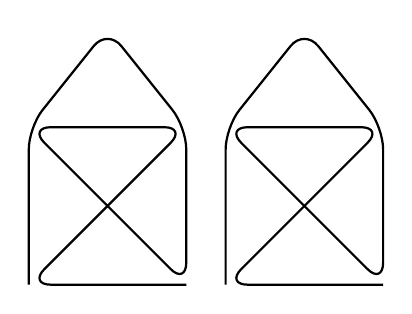
\begin{tikzpicture}
  \draw[thick,rounded corners=8pt]
    (0,0) -- (0,2) -- (1,3.25) -- (2,2) -- (2,0)
     -- (0,2) -- (2,2) -- (0,0) -- (2,0);
  \tcbpatcharcangular
  \draw[thick,rounded corners=8pt,xshift=2.5cm]
    (0,0) -- (0,2) -- (1,3.25) -- (2,2) -- (2,0)
     -- (0,2) -- (2,2) -- (0,0) -- (2,0);
\end{tikzpicture}
\end{dispExample*}

\end{docCommand}


\begin{docCommand}[doc new=2014-05-05]{tcbpatcharcround}{}
This macro reverts \refCom{tcbpatcharcangular}, i.e., the patch from
\refCom{tcbpatcharcangular} is replaced by the original code.
\end{docCommand}


\clearpage
\subsection{Extracting Node Dimensions}
The following auxiliary macros are defined by the \mylib{skins} library.
They allow to determine the width and height of an arbitrary \tikzname\ node.
To be more specific, they determine the east-to-west and the north-to-south dimensions
which may be not the maximal dimensions for a non-rectangular node.
Note that the following dimensions are measured exactly including the line width
of the border line. If a new rectangle or node with the same dimensions
and a border is to be drawn, this border width has to be substracted.

\begin{docCommand}[doc new=2014-09-19]{tcbsettowidthofnode}{\marg{register}\marg{node}}
  Sets the east-to-west dimension of the given \meta{node}
  to the \TeX\ \meta{register}.
\end{docCommand}

\begin{docCommand}[doc new=2014-09-19]{tcbsetmacrotowidthofnode}{\marg{macro}\marg{node}}
  Defines \meta{macro} as the east-to-west dimension of the given \meta{node}.
\end{docCommand}

\begin{docCommand}[doc new=2014-09-19]{tcbsettoheightofnode}{\marg{register}\marg{node}}
  Sets the north-to-south dimension of the given \meta{node}
  to the \TeX\ \meta{register}.
\end{docCommand}

\begin{docCommand}[doc new=2014-09-19]{tcbsetmacrotoheightofnode}{\marg{macro}\marg{node}}
  Defines \meta{macro} as the north-to-south dimension of the given \meta{node}.
\end{docCommand}

\begin{dispExample}

\begin{tikzpicture}
  \node[align=center,draw=red,fill=yellow] (A) {This is my\\example node};
  \tcbsetmacrotowidthofnode\mywidth{A}
  \tcbsetmacrotoheightofnode\myheight{A}
  \path[fill=blue!25!white]           %  rectangle widthout border
    ([xshift=2mm]A.south east)
    rectangle node{Copy} +(\mywidth,\myheight);
  \node[draw=blue,fill=blue!25!white, % standard border width 0.4pt
    minimum width=\mywidth-0.4pt,     % minus width of border
    minimum height=\myheight-0.4pt    % minus height of border
    ]
    at ([xshift=5cm]A) {Copy 2};
\end{tikzpicture}
\end{dispExample}


\subsection{Hyper Nodes}
The following auxiliary macro is defined by the \mylib{skins} library.
\enlargethispage*{1cm}

\begin{docCommand}[doc new=2016-02-03]{tcbhypernode}{\marg{macro}\marg{node}}
%  Sets the east-to-west dimension of the given \meta{node}
%  to the \TeX\ \meta{register}.
  Applies a hyperlink creating \meta{macro} from the package |hyperref| \cite{rahtz:hyperref}
  to an existing |tikz| \meta{node}. \refCom{tcbhypernode} can only
  be used inside a |tikzpicture| environment.
  The last argument of the \meta{macro} is to be omitted and should stand
  for an object (text) which is to be made a hyperlink.
  For example, use  |\hyperref[name]| instead of |\hyperref[name]{text}|.

\begin{dispExample}
% \usepackage{hyperref}

\begin{tikzpicture}
  \node[align=center,draw=red,fill=red!5] (mybutton)
    {Click me to jump to Section~\ref*{sec:tikzimagefilling}};
  \tcbhypernode{\hyperref[sec:tikzimagefilling]}{mybutton}
\end{tikzpicture}
\end{dispExample}

\end{docCommand}

